\documentclass[14pt]{thapathali}

% ============================================
% CUSTOMIZABLE VARIABLES - Edit these
% ============================================
\projecttitle{HYPERHEURISTIC OPTIMIZATION OF UNIVERSITY COURSE TIMETABLING PROBLEM USING REINFORCEMENT LEARNING AND GENETIC ALGORITHM}
\projectsubtitle{Final Defense Presentation}

\newcommand{\studentone}{Student Name 1}
\newcommand{\rollone}{THA080BCT002}
\newcommand{\studenttwo}{Student Name 2}
\newcommand{\rolltwo}{THA080BCT002}
\newcommand{\studentthree}{Student Name 3}
\newcommand{\rollthree}{THA080BCT002}
\newcommand{\studentfour}{Student Name 4}
\newcommand{\rollfour}{THA080BCT002}

\presentername{\studentone}
\studentroll{\rollone}
\supervisorname{Dr. Supervisor Name}
\supervisortitle{Associate Professor}
\departmentname{Department of Electronics and Computer Engineering}
\institutionname{Institute of Engineering, Thapathali Campus}
\presentationdate{\today}
\academicyear{Academic Year: 2024/2025}

% ============================================
% TITLE PAGE SETUP
% ============================================
\csname title\endcsname[\ProjectTitle]{\ProjectTitle}
\subtitle{\ProjectSubtitle}
\author[\studentone]{\studentone, \studenttwo, \studentthree, \studentfour}
\institute[\DepartmentName]{\DepartmentName}
\date[\PresentationDate]{\PresentationDate}

% ============================================
% DOCUMENT BEGINS
% ============================================
\begin{document}

% ============================================
% TITLE SLIDE
% ============================================
\begin{frame}[plain]
    \vspace{0.8cm}

    \begin{center}
        % Corrected variable: \MyProjectTitle
        {\Large \bfseries \MakeUppercase{\MyProjectTitle} \par}
    \end{center}

    \vspace{1em}

    \begin{columns}[t, onlytextwidth]
        \begin{column}{0.55\textwidth}
            \hspace{1em}{\normalsize \bfseries Team Members:}\par
            \vspace{0.3em}
            \hspace{1em}{\small \studentone{} (\rollone)}\\[2pt]
            \hspace{1em}{\small \studenttwo{} (\rolltwo)}\\[2pt]
            \hspace{1em}{\small \studentthree{} (\rollthree)}
            % ४ जना भए मात्र यो अन-कमेन्ट गर्ने:
            % \\[2pt] \hspace{1em}{\small \studentfour{} (\rollfour)}
        \end{column}

        \begin{column}{0.4\textwidth}
            \raggedleft
            {\normalsize \bfseries Supervised By:}\par
            \vspace{0.3em}
            % Corrected variables: \MySupervisor and \supervisortitle
            {\small \MySupervisor}\par
            {\footnotesize \supervisortitle}\par
        \end{column}
    \end{columns}

    \vfill

    \begin{center}
        {\normalsize \MyDeptName}\par
        {\normalsize \MyInstName}\par
        \vspace{0.3em}
        {\normalsize \MyPresDate}
    \end{center}

    \vspace{0.5cm}
\end{frame}

% ============================================
% PRESENTATION OUTLINE
% ============================================
\begin{frame}{Presentation Outline}
    \begin{columns}[t, onlytextwidth]
        \begin{column}{0.48\textwidth}
            \begin{itemize}
                \item Motivation
                \item Introduction
                \item Objectives
                \item Literature Review
                \item Scope Of Project
            \end{itemize}
        \end{column}
        \begin{column}{0.48\textwidth}
            \begin{itemize}
                \item Methodology
                \item Expected Results
                \item Feasibility Analysis
                \item Future Enhancements
                \item Conclusion
            \end{itemize}
        \end{column}
    \end{columns}
\end{frame}
% ============================================
% MOTIVATION
% ============================================
\begin{frame}{Motivation}
    \begin{itemize}
        \item GPS signal failures in deep Himalayan valleys due to topographic shielding and steep peaks.
        \item Life-threatening safety hazards for lost trekkers and rescue teams in high-altitude terrain.
        \item Critical requirement for reliable offline navigation backup on standard smartphones.
        \item Permanent and unique mountain skylines as robust geometric references for positioning.
    \end{itemize}
\end{frame}
% ============================================
% INTRODUCTION
% ============================================
\begin{frame}{Introduction}
    \begin{itemize}
        \item Satellite navigation signals weaken or vanish in steep terrain due to multi-path interference.
        \item Mountain silhouettes remain visible from open viewpoints and vary uniquely with position.
        \item Offline visual positioning system matching captured skylines to synthetic terrain databases.
        \item Focus on Khumbu region utilizing Copernicus GLO-30 Digital Elevation Models (DEM).
    \end{itemize}
\end{frame}
% ============================================
% OBJECTIVES
% ============================================

\begin{frame}{Objectives}
    \vspace{1em}
    \begin{itemize}
        \item To generate a 360-degree horizon database using the Copernicus GLO-30 Digital Elevation Model (DEM).
        \vspace{1em}
        \item To develop a matching pipeline using Euclidean distance and Dynamic Time Warping (DTW) to resolve geographic coordinates from photographs.
    \end{itemize}
\end{frame}
% ============================================
% LITERATURE REVIEW
% ============================================

\begin{frame}{Literature Review}
    \begin{table}
        \centering
        \small % अक्षर ठिक्कको साइजमा राख्न
        \caption{Summary of existing skyline geolocation approaches}
        \vspace{0.5em}
        \resizebox{\textwidth}{!}{%
            \begin{tabular}{lllc}
                \toprule
                \textbf{Authors} & \textbf{Year} & \textbf{Terrain} & \textbf{Matching Method} \\
                \midrule
                Baboud et al. & 2011 & Alps & Edge cross-correlation \\
                Baatz et al.  & 2012 & Alps (Switzerland) & Bag-of-curves \\
                Saurer et al. & 2016 & Alps & Contours + DTW \\
                Pan et al.    & 2020 & China (hilly) & Euclidean + heatmap \\
                Tomešek et al.& 2022 & Alps & Synthetic rendering \\
                \midrule
                \textbf{This Work} & \textbf{2026} & \textbf{Khumbu, Nepal} & \textbf{FFT + DTW} \\
                \bottomrule
            \end{tabular}
        }
    \end{table}
    
    \vspace{1em}
    \begin{itemize}
        \item \small \textbf{Research Gap:} Existing systems focus on European/Chinese terrain; none address the extreme elevation and GPS failure challenges in the \textbf{Himalayas}.
    \end{itemize}
    
\end{frame}
% ============================================
% SCOPE OF PROJECT
% ============================================

\begin{frame}{Scope Of Project}
    \begin{itemize}
        \item \textbf{Study Area:} A $40 \text{ km} \times 30 \text{ km}$ region in the Khumbu Valley, Nepal.
        
        \item \textbf{Geographical Boundaries:}
            \begin{itemize}
                \item \small \textbf{NW:} $86.582^\circ E, 28.041^\circ N \quad$ \textbf{NE:} $86.989^\circ E, 28.041^\circ N$
                \item \small \textbf{SW:} $86.582^\circ E, 27.770^\circ N \quad$ \textbf{SE:} $86.989^\circ E, 27.770^\circ N$
            \end{itemize}
            
        \item \textbf{Target Device:} Optimized for offline use on standard portable smartphones.
        
        \item \textbf{Operational Limit:} Requires a visible skyline; ineffective during extreme weather (dense fog/clouds) that completely blocks the horizon.
    \end{itemize}
\end{frame}
% ============================================
% PROJECT APPLICATIONS
% ============================================

\begin{frame}{Project Applications}
    \begin{itemize}
        \item \textbf{Search and Rescue (SAR):} Assisting rescue teams in locating lost trekkers or climbers in deep valleys where GPS and cellular signals are unavailable.
        
        \item \textbf{Offline Tourist Navigation:} Providing a battery-efficient and data-free navigation backup for tourists traveling in remote Himalayan regions.
        
        \item \textbf{GNSS-Denied Navigation:} Serving as a robust alternative for positioning in environments where satellite signals are blocked by steep terrain.
        
        \item \textbf{Environmental Monitoring:} Aligning historical mountain photographs with terrain models to study changes like glacier retreat and landscape shifts.
    \end{itemize}
\end{frame}
% ============================================
% METHODOLOGY
% ============================================

\begin{frame}{Methodology - [1] (System Block Diagram)}
    \begin{center}
        \vspace{1em}
        % Changed from .tex to .png
        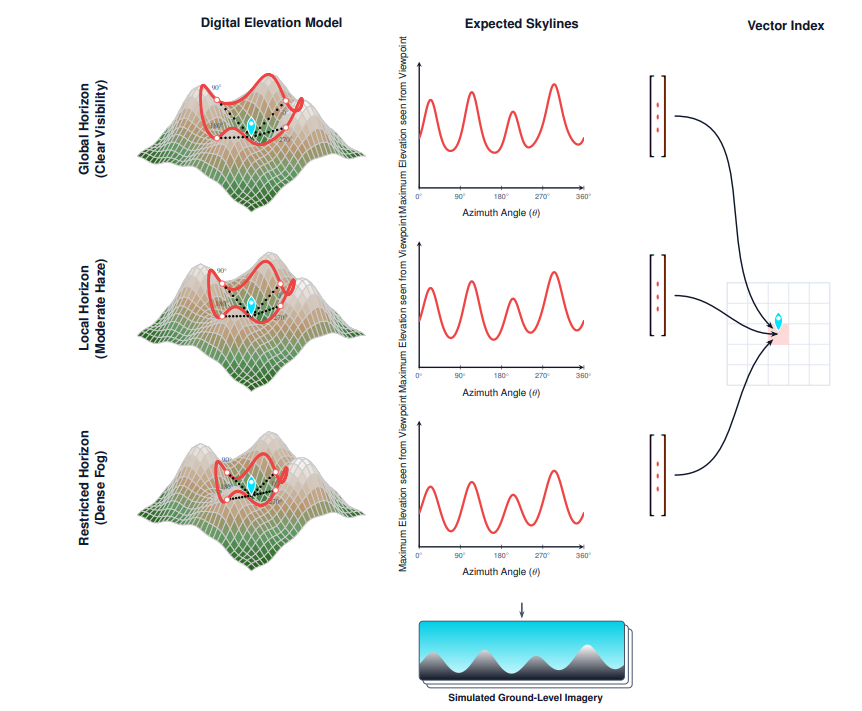
\includegraphics[width=0.85\textwidth]{src/images/page1.png} 
        \par \vspace{0.5em}
        \small \textbf{System Block Diagram:} Overview of the database generation and matching pipeline.
    \end{center}
\end{frame}

\begin{frame}{Methodology - [2] (Working Principle)}
    \begin{itemize}
        \item \textbf{Geometric Uniqueness:} Mountain skylines are permanent and unique landmarks that encode the observer's position.
        \item \textbf{Database-Query Matching:} The system matches the skyline extracted from a photo against a pre-computed database of synthetic horizons.
        \item \textbf{Offline Execution:} Coordinates are resolved by local search within the device without needing GPS or cellular data.
        \item \textbf{Absolute Elevation Signal:} Uses raw elevation values which carry strong discriminative signals for accurate positioning.
    \end{itemize}
\end{frame}

\begin{frame}{Methodology - [3] (Operational Workflow)}
    \begin{itemize}
        \item \textbf{Step 1 (Pre-processing):} Synthesis of 360-degree horizon profiles from DEM using ray-casting.
        \item \textbf{Step 2 (Segmentation):} Detecting sky-terrain boundary using a U-Net model.
        \item \textbf{Step 3 (Matching):} Fast global search using FFT-based Euclidean distance.
        \item \textbf{Step 4 (Refinement):} Fine-tuning the best candidates using Dynamic Time Warping (DTW).
        \item \textbf{Step 5 (Output):} Returning predicted Lat/Long and camera heading.
    \end{itemize}
\end{frame}

\begin{frame}{Methodology - [4] (Flow Of Proposed System)}
    \begin{center}
        \vspace{0.5em}
        % Changed from .tex to .png
        % Used height constraint here because flowcharts are often tall
        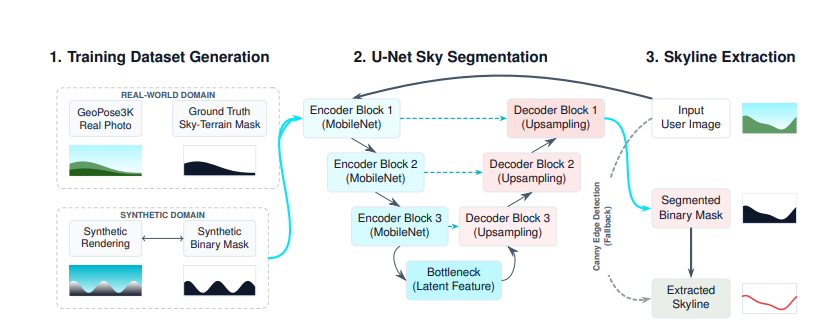
\includegraphics[height=0.7\textheight]{src/images/page2.png} 
        \par \vspace{0.5em}
        \small \textbf{Flowchart:} Pipeline from raw photo input to extracted skyline mask.
    \end{center}
\end{frame}

\begin{frame}{Methodology - [5] (Hardware Requirement)}
    \begin{itemize}
        \item \textbf{Training Host:} Workstation with CUDA-enabled GPU for training the segmentation model.
        \item \textbf{Deployment Target:} Mid-range Android smartphone for offline search.
        \item \textbf{Storage:} ~80 MB RAM/Disk space for storing 4,800 horizon viewpoints.
        \item \textbf{Camera:} Standard smartphone camera for image acquisition.
    \end{itemize}
\end{frame}

\begin{frame}{Methodology - [6] (Software Requirement)}
    \begin{itemize}
        \item \textbf{Programming Language:} Python (Development), C++ (Android Deployment).
        \item \textbf{ML Libraries:} PyTorch (Model training), NumPy/SciPy (Signal processing).
        \item \textbf{Computer Vision:} OpenCV for image manipulation and edge detection.
        \item \textbf{Libraries:} HORAYZON (Ray-casting), Android NDK (Deployment).
    \end{itemize}
\end{frame}

\begin{frame}{Methodology - [7] (Machine Learning Architecture)}
    \begin{itemize}
        \item \textbf{Model:} U-Net architecture for robust binary segmentation.
        \item \textbf{Encoder:} MobileNet-V3 backbone for lightweight and fast processing.
        \item \textbf{Objective:} To segment query photographs into sky and terrain masks even under poor lighting.
        \item \textbf{Fallback:} Canny Edge detection for low-confidence outputs.
    \end{itemize}
\end{frame}

\begin{frame}{Methodology - [8] (Algorithm Architecture)}
    \begin{center}
        \vspace{1em}
        % Changed from .tex to .png
        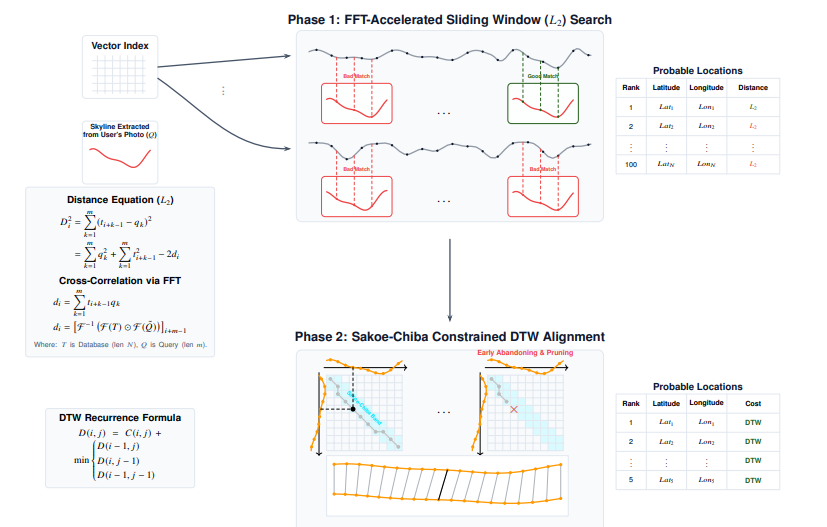
\includegraphics[width=0.9\textwidth]{src/images/page3.png} 
        \par \vspace{0.5em}
        \small \textbf{Algorithm Architecture:} Two-stage engine showing FFT-Sliding Window and DTW refinement.
    \end{center}
\end{frame}

\begin{frame}{Methodology - [9] (Dataset Preparation)}
    \begin{itemize}
        \item \textbf{Real Data:} GeoPose3K (3,000 labeled alpine images) for pre-training.
        \item \textbf{Synthetic Data:} Khumbu renderings generated from Copernicus GLO-30 DEM.
        \item \textbf{Ground Truth:} 45,000+ geotagged panoramas from Google Street View's Everest Trail.
        \item \textbf{Augmentation:} Procedural fog textures to simulate Himalayan weather.
    \end{itemize}
\end{frame}

\begin{frame}{Methodology - [10] (Snapshot of Dataset)}
    \begin{center}
        \vspace{1em}
        % You can also use an image here if you have one (e.g. dataset_sample.png)
        \fbox{\parbox{0.8\textwidth}{\centering
                \vspace{1cm}
                \textbf{GeoPose3K \& Khumbu Synthetic Images}\\
                \vspace{0.5em}
                (Input Image $\rightarrow$ Binary Mask $\rightarrow$ Skyline Vector)
                \vspace{1cm}
            }}
        \par \small \textbf{Snapshot:} Examples of the sky-terrain segmentation training data.
    \end{center}
\end{frame}

\begin{frame}{Methodology - [11] (Model Training)}
    \begin{itemize}
        \item \textbf{Strategy:} Pre-training on alpine data and fine-tuning on synthetic Khumbu terrain.
        \item \textbf{Optimization:} Adam optimizer with Cross-Entropy loss for pixel-level classification.
        \item \textbf{Evaluation:} Accuracy measured by grid-cell assignment on the test set.
        \item \textbf{Generalization:} Train/test splits made at the panorama level to avoid data leakage.
    \end{itemize}
\end{frame}
% ============================================
% EXPECTED RESULTS
% ============================================

\begin{frame}{Expected Results - [1] (Output Interface)}
    \begin{center}
        % Standard size for the main result image
        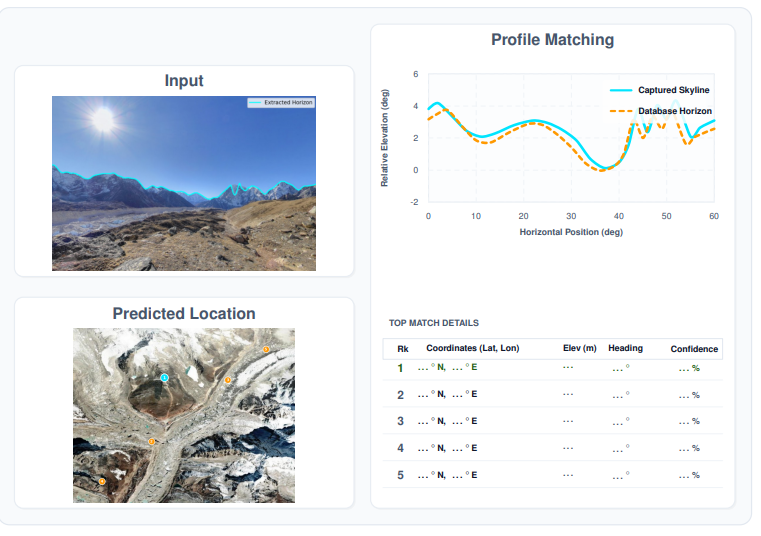
\includegraphics[width=0.85\textwidth, height=0.7\textheight, keepaspectratio]{src/images/page4.png} 
        \vfill
        \small \textbf{Figure:} Proposed interface showing predicted location on map and profile alignment.
    \end{center}
\end{frame}

\begin{frame}{Expected Results - [2] (Performance Metrics)}
    \begin{columns}[t, onlytextwidth]
        \begin{column}{0.55\textwidth}
            \textbf{Metrics for Evaluation:}
            \begin{itemize}
                \item \textbf{Top-$k$ Accuracy:} How often the ground-truth location appears in the top $1, 5, \text{ or } 10$ candidates.
                \item \textbf{Heading Error:} Angular difference between predicted and actual camera direction (limit: $\pm 0.25^\circ$).
                \item \textbf{Latency:} Time taken for FFT search and DTW refinement (Target: $< 2$ seconds).
            \end{itemize}
        \end{column}
        \begin{column}{0.42\textwidth}
            \begin{center}
                % If you have a PNG for this graph later, replace this \fbox with \includegraphics
                \fbox{\parbox{0.9\textwidth}{\centering
                    \vspace{1.5cm}
                    \small \textbf{[Expected Accuracy Graph]}\\
                    \tiny (Top-$k$ vs Success Rate)
                    \vspace{1.5cm}
                }}
            \end{center}
        \end{column}
    \end{columns}
\end{frame}

\begin{frame}{Expected Results - [3] (Robustness Analysis)}
    \begin{itemize}
        \item \textbf{Weather Resistance:} Performance evaluation across different visibility tiers (Clear, Moderate Haze, Dense Fog).
        \item \textbf{Focal Length Tolerance:} DTW's ability to handle stretching/compression from different smartphone lenses.
        \item \textbf{Memory Footprint:} Maintaining the $\sim 79$ MB database entirely in RAM for fast access.
    \end{itemize}
\end{frame}
% ============================================
% ANALYSIS
% ============================================

\begin{frame}{Analysis}
    \textbf{Data Analysis:}
    \begin{itemize}
        \item Analysis point 1: Key observation from the data
        \item Analysis point 2: Consistency and reliability of measurements
        \item Analysis point 3: Statistical summary of results
        \item Analysis point 4: Comparison with expected values
        \item Analysis point 5: Data logging and storage observations
    \end{itemize}
\end{frame}

\input{src/slides/13-future-enhancements.tex}
% ============================================
% CONCLUSION
% ============================================

\begin{frame}{Conclusion}
    \begin{itemize}
        \item Conclusion point 1: Summary of the proposed/developed system
        \item Conclusion point 2: Key contributions and significance
        \item Conclusion point 3: Feasibility and approach taken
        \item Conclusion point 4: Results achieved or expected outcomes
        \item Conclusion point 5: Practical impact and relevance
    \end{itemize}
\end{frame}

% ============================================
% REFERENCES
% ============================================

\begin{frame}{References}
    \begin{itemize}
        \item Reference 1: Author(s), ``Title of paper/article,'' Journal/Conference, Date. Available: URL. [Accessed: Date]

        \item Reference 2: Author(s), ``Title of paper/article,'' Journal/Conference, vol. X, no. Y, pp. XX--YY, Year
    \end{itemize}
\end{frame}

\begin{frame}{References(Contd..)}
    \begin{itemize}
        \item Reference 3: Author(s), ``Title of paper/article,'' Journal/Conference, vol. X, p. XXXXX, Month. Year

        \item Reference 4: Author(s), ``Title of paper/article,'' Journal/Conference, vol. X, no. Y, pp. XX--YY, Year
    \end{itemize}
\end{frame}


\end{document}
